\documentclass{article}

\usepackage[dblblindworkshop, final]{neurips_2026}
\workshoptitle{TAE (Trust-AI-Eval): Can We Trust AI Evaluation?}

\usepackage[utf8]{inputenc}
\usepackage[T1]{fontenc}
\usepackage[hypertexnames=false]{hyperref}
\hypersetup{
  pdfauthor={Polina Korobeinikova, Dmitry Lvov, and Ilya Pershin},
  pdftitle={Similar Scores, Different High-Risk Episodes: Auditing Model Selection in Longitudinal EHRs},
  pdfsubject={TAE (Trust-AI-Eval): Can We Trust AI Evaluation?},
  pdfkeywords={trustworthy evaluation, longitudinal EHRs, model selection, calibration, stability},
  pdfcreator={LaTeX},
  pdfproducer={}
}
\usepackage{xurl}
\usepackage{booktabs}
\usepackage{amsmath}
\usepackage{amsfonts}
\usepackage{microtype}
\usepackage{xcolor}
\usepackage{graphicx}
\usepackage{multirow}
\usepackage{array}
\usepackage{placeins}
\usepackage{tikz}
\usetikzlibrary{arrows.meta,positioning,decorations.pathreplacing}

\definecolor{auditnavy}{HTML}{17324D}
\definecolor{auditblue}{HTML}{0072B2}
\definecolor{auditorange}{HTML}{D55E00}

\title{Similar Scores, Different High-Risk Episodes: Auditing Model Selection in Longitudinal EHRs}

\author{
  Polina Korobeinikova$^{1}$ \quad Dmitry Lvov$^{1,2}$ \quad Ilya Pershin$^{1,3}$\\
  $^{1}$Research Center of the Artificial Intelligence Institute, Innopolis University, Innopolis, Russia\\
  $^{2}$ITMO University \quad $^{3}$Kazan Federal University
}

\newcommand{\raw}{\textsc{Raw}}
\newcommand{\era}{\textsc{Era}}
\newcommand{\topten}{top-10\%}
\newcommand{\ci}{95\% CI}

\begin{document}

\maketitle

\begin{abstract}
Clinical prediction pipelines are commonly selected by small differences in
aggregate held-out scores, although operational prioritization depends on
calibrated risks, retraining stability, and which episodes fill the chosen
capacity. Longitudinal EHRs make this problem acute: repeated diagnoses can
represent persistent disease or redundant documentation, and compressing them
can change both prediction quality and the history visible to a model. We
compare Raw histories with a persistence-aware Era+backfill representation on
EHRSHOT 30-day readmission and ICU-transfer using a decision-aware evaluation
of cohort performance, uncertainty, calibration, retraining, selected sets,
and controlled repetition. Across five-seed ensembles at 4,096 events,
Era+backfill records the better observed value in all ten conventional
task--metric comparisons, although every paired patient-cluster interval
includes zero. At the same top-decile capacity, it captures three additional
readmission positives and one additional ICU positive while replacing 34
(15.5\%) and 51 (25.0\%) episodes in each prioritized set. These replacements
remain after five-seed ensembling, while within-representation single-seed
comparisons also show substantial variability. A structure-matched control
locates the clearest ICU gains in explicit persistence state, while controlled
diagnosis repetition reverses the sensitivity ordering across tasks. Aggregate rankings therefore
neither determine whom a pipeline prioritizes nor separate representation
effects from retraining instability. A joint evaluation profile makes those
model-selection consequences visible. Code and publication-safe aggregates are
available at \url{https://github.com/LvovDmitro/ehrshot-state-or-space}.
\end{abstract}

\section{Introduction}

Clinical risk models influence which records receive attention and which
patients are prioritized for follow-up. Yet representation choices are often
advanced on a small difference in one held-out metric. This practice assumes
that the same choice remains favorable under other clinically relevant metrics,
repeated training, calibration assessment, and the threshold used to prioritize
cases.

Longitudinal electronic health records (EHRs) make this assumption especially
consequential. A patient timeline may contain thousands of irregular events and
the same diagnosis repeated across visits. A Raw suffix preserves the recorded
stream, whereas a persistence-aware representation can summarize repeated
diagnoses as explicit condition states and use the released context positions
for earlier history. Comparing these representations with one held-out score
captures average prediction quality, but says little about whether they rank
the same episodes or respond similarly to repeated documentation.

We examine this gap on the EHRSHOT 30-day readmission and ICU-transfer tasks
\citep{wornow2023ehrshot}. Figure~\ref{fig:headline} previews the central result.
Our evaluation profile connects predictive metrics,
paired patient-cluster uncertainty, calibration, patient weighting, complete
retraining, top-decile set agreement, and response to a strictly
pre-prediction perturbation. Era+backfill leads all ten primary
episode-weighted point estimates, but the paired intervals retain uncertainty
and fixed-capacity prioritization differs. Component controls examine explicit
state encoding; frozen-pipeline repetition tests probe behavioral sensitivity.

\begin{figure}[t]
  \centering
  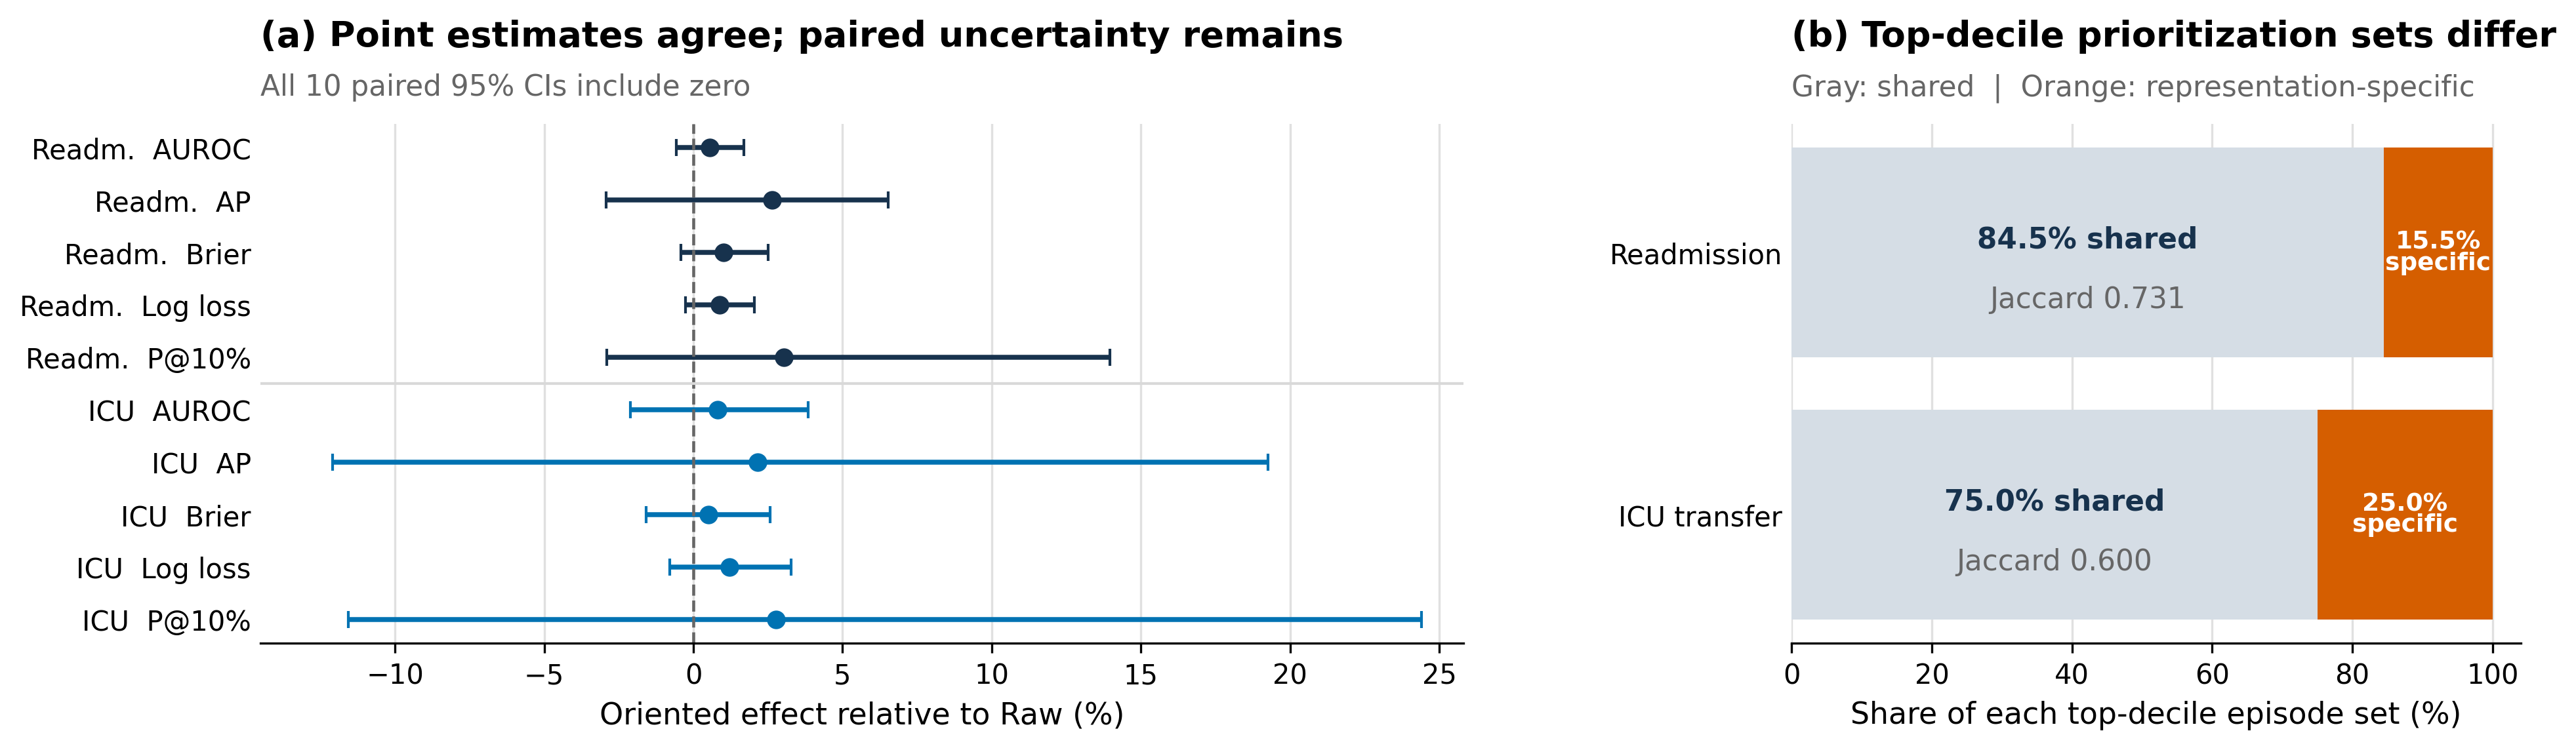
\includegraphics[width=0.98\linewidth]{figure_decision_gap.png}
  \caption{Aggregate direction, paired uncertainty, and top-decile set
  disagreement. Panel (a) shows oriented effects relative to Raw with paired
  patient-cluster 95\% intervals: all ten point estimates favor Era+backfill,
  while every interval crosses zero. Panel (b) shows that 15.5\% of each
  readmission top-decile set and 25.0\% of each ICU set is
  representation-specific.}
  \label{fig:headline}
\end{figure}

\FloatBarrier

\section{Related Work}

\paragraph{Longitudinal EHR representations.}
RETAIN established reverse-time modeling of clinical sequences
\citep{choi2016retain}; EHRSHOT later standardized patient-level prediction
tasks \citep{wornow2023ehrshot}, and MEDS provided a common event-stream format
\citep{meds2024}. \emph{Context Clues} varies context length from 512 to 16,384
tokens on EHRSHOT and studies performance across naturally occurring
copy-forward repetition, irregular timing, and disease progression
\citep{wornow2025context}. These studies establish the importance of history
length and repeated documentation, but leave two mechanisms entangled under a
fixed event budget: encoding repeated diagnoses as persistent state and using
positions released by compression to admit earlier history. Consequently, the
source of any representation-level difference remains difficult to identify.

\paragraph{Reliable evaluation of clinical prediction.}
Clinical prediction guidance distinguishes discrimination, calibration, and
intended use, and calls for transparent reporting of data splits and model
development \citep{vancalster2019calibration,collins2024tripod}. Average
precision (AP) is
particularly informative for rare outcomes \citep{saito2015precision}, while
problem-aware validation frameworks emphasize metric portfolios rather than a
single default score \citep{maierhein2024metrics}. These practices improve the
assessment of a fixed model, but they do not by themselves reveal whether a
representation choice is stable across analysis units and retraining.

\paragraph{Underspecification and behavioral stability.}
Models with similar held-out performance can encode different solutions
\citep{damour2022underspecification}, and repeated EHR training can alter
patient-level risk assignments while preserving aggregate metrics
\citep{lopezmartinez2022instability}. Benchmark reuse can further distort model
selection \citep{dwork2015holdout,westphal2019test,cawley2010selection}, while
copy-forward documentation motivates behavioral tests of repeated information
\citep{thornton2013copy}. Together, these strands leave open whether a
representation preference remains stable across analysis units, retraining
runs, calibration summaries, selected episodes, and structured perturbations.

\section{Methodology}

We compare Raw and Era+backfill under a common protocol comprising
patient-disjoint prediction tasks, fixed task-specific architectures,
seed-wise calibration on tuning data, and held-out evaluation at both cohort
and top-decile levels. Figure~\ref{fig:methodology} illustrates the
representation transformation and shared evaluation pipeline.

\begin{figure}[t]
  \centering
  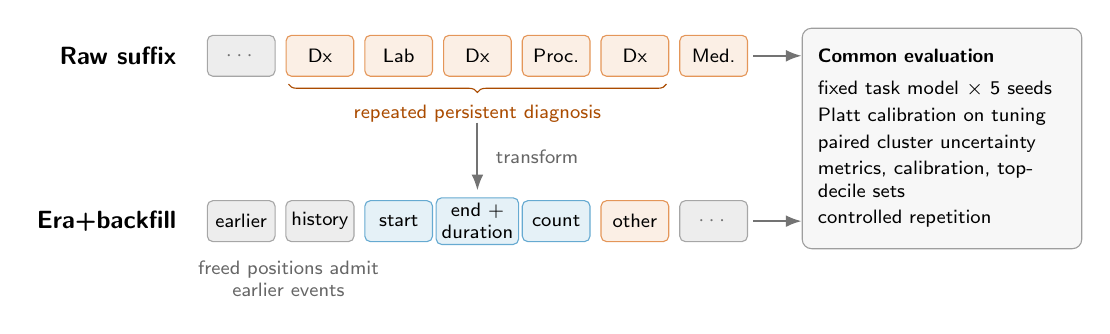
\begin{tikzpicture}[
    font=\sffamily\scriptsize,
    token/.style={draw=black!35, rounded corners=.7mm, minimum width=.86cm,
      minimum height=.52cm, inner sep=2pt, align=center},
    rawtoken/.style={token, fill=auditorange!10, draw=auditorange!65},
    eratoken/.style={token, fill=auditblue!10, draw=auditblue!60},
    earlytoken/.style={token, fill=black!7, draw=black!35},
    eval/.style={draw=black!38, fill=black!3, rounded corners=1.2mm,
      minimum width=3.55cm, minimum height=2.8cm, text width=3.15cm,
      inner sep=5pt, align=left},
    flow/.style={-{Latex[length=2mm]}, line width=.75pt, color=black!55}
  ]
    \node[anchor=east, font=\sffamily\small\bfseries] at (-5.25,1.05) {Raw suffix};
    \node[earlytoken, text=black!55] at (-4.55,1.05) {$\cdots$};
    \node[rawtoken] at (-3.55,1.05) {Dx};
    \node[rawtoken] at (-2.55,1.05) {Lab};
    \node[rawtoken] at (-1.55,1.05) {Dx};
    \node[rawtoken] at (-.55,1.05) {Proc.};
    \node[rawtoken] at (.45,1.05) {Dx};
    \node[rawtoken] at (1.45,1.05) {Med.};
    \draw[decorate, decoration={brace, mirror, amplitude=3pt},
      auditorange!80!black] (-3.95,.69) -- (.85,.69)
      node[midway, below=4pt, text=auditorange!80!black]
      {repeated persistent diagnosis};

    \node[anchor=east, font=\sffamily\small\bfseries] at (-5.25,-1.05)
      {Era+backfill};
    \node[earlytoken] at (-4.55,-1.05) {earlier};
    \node[earlytoken] at (-3.55,-1.05) {history};
    \node[eratoken] at (-2.55,-1.05) {start};
    \node[eratoken] at (-1.55,-1.05) {end +\\duration};
    \node[eratoken] at (-.55,-1.05) {count};
    \node[rawtoken] at (.45,-1.05) {other};
    \node[earlytoken, text=black!55] at (1.45,-1.05) {$\cdots$};
    \draw[flow] (-1.55,.2) -- (-1.55,-.66)
      node[midway, right=3pt, text=black!60] {transform};
    \node[anchor=north, align=center, text=black!60] at (-3.95,-1.43)
      {freed positions admit\\earlier events};

    \node[eval] (audit) at (4.35,0)
      {\textbf{Common evaluation}\\[1.2mm]
       fixed task model $\times$ 5 seeds\\[.6mm]
       Platt calibration on tuning\\[.6mm]
       paired cluster uncertainty\\[.6mm]
       metrics, calibration, top-decile sets\\[.6mm]
       controlled repetition};
    \draw[flow] (1.95,1.05) -- (audit.west |- 0,1.05);
    \draw[flow] (1.95,-1.05) -- (audit.west |- 0,-1.05);
  \end{tikzpicture}
  \caption{Representation mechanism and common evaluation. Raw preserves
  repeated diagnosis events. Era encodes start, end-with-duration, and count;
  compression can admit earlier events under the same $L$-event budget. Both
  representations then enter the same task-specific training, calibration,
  and evaluation protocol.}
  \label{fig:methodology}
\end{figure}

\subsection{Data and prediction tasks}

We use EHRSHOT 30-day readmission and ICU-transfer prediction
\citep{wornow2023ehrshot,ehrshotrepo2026}. Readmission is predicted at 23:59 on
the discharge day, with outcomes measured over the following 30 days; ICU
transfer is predicted at 23:59 on the admission day. The benchmark provides
patient-disjoint train, tuning, and held-out assignments. The held-out cohorts
contain 2,189 episodes from 1,190 patients for readmission (260 positives) and
2,037 episodes from 1,154 patients for ICU transfer (85 positives); complete
split counts appear in Appendix~\ref{app:data_details}.

For episode $i$, let $\tau_i$ denote prediction time and $g_i$ its patient. The
available history is
\begin{equation}
H_i(\tau_i)=\{(c_{ij},t_{ij},x_{ij}):t_{ij}\leq\tau_i\},
\end{equation}
where $c_{ij}$ is an event code and $x_{ij}$ contains optional numeric values.
The split audit verified unique episode assignment, patient separation, label
coverage, and agreement with the official subject split.

\subsection{Persistence-aware histories}

We derive the set of candidate persistent diagnoses using only patients
assigned to train. A code qualifies if it occurs in at least 50 training
patients and at least half have records on multiple days. It must also satisfy
one of two span criteria: at least 10\% of patients span 365 days, or the 75th
percentile of patient-level spans is at least 365 days. This fixed rule selects
239 of 6,736 diagnosis codes among 2,094 training patients with diagnosis
events. The vocabulary and numeric normalization statistics are also fit only
on the training split.

The held-out patients therefore play no role in defining the persistent-code
set $S$. The Raw representation retains the most recent $L$ events, whereas
Era+backfill first transforms the complete available history and then takes
the same-length suffix:
\begin{equation}
R_i^{\mathrm{Raw}}=\operatorname{suffix}_L(H_i),\qquad
R_i^{\mathrm{Era}}=\operatorname{suffix}_L(T_{90,S}(H_i)).
\end{equation}
We use $L=4096$ for the primary comparison and $L=16384$ for context-length
sensitivity. At $L=4096$, 53.5\% of readmission histories and 41.9\% of ICU
histories are truncated across all splits.

For each selected diagnosis, duplicate mentions are first summarized by visit
day. Consecutive mentions separated by at most 90 days form one condition era.
An era with at least two diagnosis points becomes three ordered tokens: a start
token, an end token carrying duration in days, and a count-bin token carrying
the number of diagnosis points. Single-point eras and all nonselected events
remain ordinary events. The full-history \textsc{Era+Backfill} variant transforms
the available history before taking the final $L$ positions, so positions freed
by compression can admit earlier events.

Unless stated otherwise, the primary \textsc{Era+Backfill} pipeline uses a
90-day gap and $L=4096$. We refer to its controls consistently as
\textsc{Era No-Backfill} and \textsc{Era Structure-Null}.

We add two controls. \textsc{Era No-Backfill} first takes the Raw $L$-event
suffix and then transforms it, prohibiting older-event admission.
\textsc{Era Structure-Null} exactly preserves the number, timestamps, ordering,
base diagnoses, and backfilled positions of \textsc{Era+Backfill}, but replaces
special state tokens by their base diagnosis and removes their state-specific
numeric values. It isolates the added explicit state encoding more closely than
a Raw comparison, although positions and timing still carry implicit
information. For ICU, we additionally evaluate 30- and 180-day era gaps.

The no-backfill comparison is a full-history transformation with backfill
versus transformation after Raw truncation. It changes older-event admission
and the histories used to construct era boundaries, durations, and counts;
only the structure-null control more directly isolates explicit state tokens.

\subsection{Models and training}

We use a numeric-aware RETAIN-lite model for readmission and a two-layer
numeric-aware GRU for ICU transfer. Each event combines a 64-dimensional token
embedding, projected temporal features, and projected numeric value/missingness
features. Hidden size is 128 and dropout is 0.20. Models use batches of eight,
AdamW ($10^{-3}$ learning rate, $10^{-4}$ weight decay), gradient clipping at
1, and binary cross-entropy with training-set positive weight
$n_{\mathrm{negative}}/n_{\mathrm{positive}}$. Training runs for at most 12
epochs; the checkpoint with the best tuning AP is restored, with early stopping
after three consecutive epochs without improvement.

Each task--representation pair is trained with seeds 42--46. A logistic
calibrator is fitted to tuning logits for each run and applied once to held-out
logits \citep{platt1999probabilistic,guo2017calibration}. We average the five
calibrated held-out probabilities to obtain
\begin{equation}
\bar p_i=\frac{1}{5}\sum_{s=1}^{5}\sigma(a_s z_{is}+b_s),
\end{equation}
where $z_{is}$ is the held-out logit for seed $s$.

\subsection{Evaluation protocol}

The primary analysis compares Raw and Era+backfill at $L=4096$ across five
held-out metrics under episode weighting. Secondary analyses examine patient
weighting, retraining stability, top-decile agreement, calibration, context and
era-horizon sensitivity, and controlled diagnosis repetition.

Development used held-out feedback across 81 variants per task, so the analysis
is retrospective. The conditional bootstrap intervals do not account for this
adaptive selection. The shared protocol directly measures aggregate performance
and agreement in episode prioritization for the fitted pipelines; it does not
estimate performance on an untouched confirmatory cohort.

\paragraph{Metrics and estimands.}

We compute AUROC, average precision (AP), Brier score, log loss, and precision
among the highest 10\% predicted risks. AP is the recall-increment-weighted mean
of precision along the precision--recall curve. AUROC measures ranking across
thresholds; AP emphasizes positive-case retrieval; Brier score and log loss
assess probability quality; and \topten{} precision measures retrieval at a
fixed top-decile capacity. We orient every paired effect so that positive favors
Era+backfill:
\begin{equation}
\Delta_m=\begin{cases}
m(\mathrm{Era})-m(\mathrm{Raw}), & \text{higher is better},\\
m(\mathrm{Raw})-m(\mathrm{Era}), & \text{lower is better}.
\end{cases}
\end{equation}

The primary estimand treats episodes equally but resamples patients as
clusters: each bootstrap sample draws patients with replacement and retains all
their episodes. We use 10,000 paired replicates and percentile \ci{}s. A
sensitivity estimand assigns each patient the same total weight,
$w_i=1/n_{g_i}$, where $n_{g_i}$ is that patient's episode count. Episodes are ranked by predicted risk,
and the boundary episode can enter fractionally so the selected total weight is
exactly 10\%. This estimand reduces the influence of patients with repeated
admissions while preserving the episode-level prediction target. These
intervals quantify held-out sampling uncertainty conditional on the fitted
five-seed ensembles; they do not include model-selection or full-retraining
uncertainty.

\paragraph{Retraining and selected-set stability.}

Under episode weighting, each pipeline selects the $k=\lceil0.10N\rceil$
highest-risk episodes from a cohort of size $N$, with deterministic
episode-identifier tie-breaking. The capacity is shared, not the probability
cutoff. For two selected sets $A$ and $B$, each of size $k$, we define
\[
J(A,B)=\frac{|A\cap B|}{|A\cup B|},\qquad
r(A,B)=\frac{|A\setminus B|}{k}=\frac{|B\setminus A|}{k}.
\]
Jaccard measures intersection relative to union; the replacement fraction $r$
measures the share of either fixed-capacity set absent from the other. For
baseline and perturbed sets, we call this fraction churn and report entered and
exited episodes separately, without counting their sum as the replacement rate.

We report metric means and standard deviations across seeds, the number of
seeds favoring each representation, and pairwise Jaccard overlap of seed-specific
\topten{} prediction-episode sets. We also compare the ensemble \topten{} sets
across Raw and Era+backfill. This distinguishes stability of global performance
from stability of selected episodes \citep{lopezmartinez2022instability}.
For matched-size references, we average calibrated probabilities over every
one- or two-seed subset. Within a representation, we compare disjoint subsets;
across representations, we compare the same seed-index subset. Sizes one and
two yield 10 and 15 within-representation pairs and 5 and 10 cross-representation
pairs, respectively. These comparisons reuse fitted models and are not
independent replicates. The five-seed cross-representation comparison is
reported separately. All seeds use the same training patients and split.

A post-hoc descriptive analysis characterizes representation-specific ensemble
selections using the repeat count for one candidate diagnosis, the time from
its first mention to prediction, and retained Raw sequence length. The candidate
is the deterministic diagnosis chosen for the stress-test plan, not a summary
of all diagnoses. Its age since first mention is neither a first-to-last
documentation span nor a condition-era duration. We report coverage because
these characteristics are available only for episodes included in that plan;
this profile is distinct from the strictly pre-prediction stress cohort.

\paragraph{Calibration and multiplicity.}

For the two primary 4,096-event representations in each task, we report
10-bin equal-frequency expected calibration error (ECE), calibration intercept
and slope, and reliability curves. We obtain uncertainty with 2,000
patient-cluster bootstrap samples. Intercept 0 and slope 1 are the targets,
complementing Brier score and log loss \citep{vancalster2019calibration}.

The full analysis tracks 12 representation contrasts across five metrics.
Holm and Benjamini--Hochberg sensitivity adjustments are applied across the
entire family of 60 contrast--metric quantities, not separately within the five
ICU state-versus-null comparisons \citep{holm1979multiple,benjamini1995fdr}.
These retrospective summaries accompany nominal patient-cluster intervals;
complete details appear in the appendix.

\paragraph{Synthetic repetition stress test.}

For each eligible held-out episode, we deterministically select one diagnosis
from the 239-code list that is already present in at least two reconstructed
visits. Later visits where that diagnosis is absent are ranked by a stable
hash. Nested subsets requested at 0\%, 25\%, 50\%, or 100\% of eligible visits
receive a duplicate diagnosis event. The requested fraction $f$ refers to
eligible visits, not all visits or events in the history. The number of changed
visits is $\lceil f n_{\mathrm{eligible}}\rceil$, so realized fractions at
25\% and 50\% can be materially higher when few visits are eligible.
The same selected diagnosis and visit subset are used for Raw and Era+backfill
pipelines. Frozen checkpoints, vocabularies, and calibrators produce new
predictions; no model is retrained.

We restrict the analysis to episodes whose eligible visits are strictly before
prediction time. This leaves 1,286
of 2,189 readmission episodes (58.7\%; 685 patients, 157 positives) and 1,028
of 2,037 ICU episodes (50.5\%; 570 patients, 37 positives). The stress-test
analysis compares the mean absolute change in calibrated
probability from the stress run's own 0\% baseline with a 10,000-sample
patient-cluster bootstrap. At the 100\% level, we also count episodes entering
and leaving each pipeline's \topten{} set, recomputed within this eligible
cohort rather than the complete held-out cohort.

For each task--pipeline pair, a post-hoc profile selects the
$n_{\mathrm{tail}}=\lceil0.05N\rceil$ largest absolute calibrated probability
shifts from the stress run's own 0\% baseline to 100\% repetition. We sort by
descending $|\Delta p|$, breaking ties by ascending episode identifier, and
compare candidate-diagnosis and eligible-visit medians with the remainder.
This tail selection is distinct from top-decile prioritization and is
conditional on the strict stress cohort.

\section{Results}
\FloatBarrier

\subsection{Primary predictive performance and paired uncertainty}

Table~\ref{tab:primary_results} reports the primary five-seed ensembles.
At $L=4096$, Era+backfill gives the better observed value in all ten
task--metric comparisons. The readmission differences are 0.0043 AUROC,
0.0108 AP, and 1.37 percentage points in P@10; the corresponding ICU
differences are 0.0065, 0.0047, and 0.49 points. This point-estimate ranking is
consistent across metrics, while every paired patient-cluster interval spans
zero. The aggregate table therefore supplies a clear observed ordering but not
a decisive representation choice on its own.

\begin{table}[!htbp]
  \caption{Primary retrospective held-out results at 4,096 events. $\Delta$ is the
  Era+backfill benefit, oriented so positive is better; intervals use paired
  patient-cluster bootstrap conditional on the fitted ensembles. Development
  reused this held-out cohort across 81 variants per task; intervals do not
  account for adaptive model selection.}
  \label{tab:primary_results}
  \centering
  \footnotesize
  \begin{tabular*}{\linewidth}{@{\extracolsep{\fill}}lrrlrrl@{}}
    \toprule
    & \multicolumn{3}{c}{Readmission} & \multicolumn{3}{c}{ICU transfer} \\
    \cmidrule(lr){2-4}\cmidrule(l){5-7}
    Metric & Raw & Era & $\Delta$ [95\% CI] & Raw & Era & $\Delta$ [95\% CI] \\
    \midrule
    AUROC & .7942 & .7985 & .0043 [$-.0045$, .0135]
      & .7948 & .8013 & .0065 [$-.0167$, .0305] \\
    AP & .4097 & .4206 & .0108 [$-.0120$, .0268]
      & .2194 & .2241 & .0047 [$-.0265$, .0422] \\
    Brier & .08690 & .08602 & .00088 [$-.00036$, .00217]
      & .03637 & .03618 & .00018 [$-.00058$, .00094] \\
    Log loss & .29956 & .29693 & .00263 [$-.00077$, .00614]
      & .14926 & .14745 & .00181 [$-.00119$, .00490] \\
    P@10\% & .4521 & .4658 & .0137 [$-.0131$, .0631]
      & .1765 & .1814 & .0049 [$-.0204$, .0431] \\
    \bottomrule
  \end{tabular*}
\end{table}

\FloatBarrier

\subsection{Component analysis of persistence-state encoding}

Table~\ref{tab:component_results} decomposes the two mechanisms. The
structure-matched control holds sequence length, timestamps, base
diagnoses, and backfilled positions fixed while removing explicit state tokens
and values. In ICU transfer, explicit state encoding improves all five observed
metrics over this control, and all five nominal paired intervals exclude zero;
the differences include 0.0309 AUROC and 0.0416 AP. The full-history
transformation with backfill also improves ICU AUROC and log loss relative to
transformation after Raw truncation, but that contrast jointly changes era
construction and older-event admission. The earliest retained timestamp moves
earlier in only 4.2\% of ICU and 5.8\% of readmission episodes, making the
structure-null comparison the more specific evidence for explicit state.

\begin{table}[!htbp]
  \caption{ICU component contrasts. Benefits are oriented so positive is
  better; intervals use paired patient-cluster bootstrap.}
  \label{tab:component_results}
  \centering
  \small
  \begin{tabular*}{\linewidth}{@{\extracolsep{\fill}}lcc@{}}
    \toprule
    Metric & State vs. structure-null & Full history vs. post-truncation \\
    \midrule
    AUROC & .0309 [.0092, .0524] & .0281 [.0102, .0475] \\
    AP & .0416 [.0049, .0908] & .0234 [$-.0091$, .0571] \\
    Brier & .00112 [.00010, .00219] & .00063 [$-.00011$, .00137] \\
    Log loss & .00783 [.00393, .01221] & .00430 [.00153, .00717] \\
    P@10\% & .0245 [.0046, .0550] & .0147 [$-.0100$, .0464] \\
    \bottomrule
  \end{tabular*}
\end{table}

Across 60 retrospective contrast--metric quantities, 12 nominal intervals
exclude zero. An approximate bootstrap sign-tail sensitivity yields three quantities below 0.05
after Holm and seven after Benjamini--Hochberg, with both adjustments applied
across all 60 quantities. Among the five ICU state-versus-null comparisons,
log loss is the only quantity below 0.05 after this family-wide Holm adjustment.
These retrospective quantities are sensitivity summaries rather than
confirmatory significance tests.

\FloatBarrier

\subsection{Context-length and era-horizon sensitivity}

At $L=16{,}384$, the preferred representation depends on task and metric
(Table~\ref{tab:sensitivity_results}). For readmission, Raw gains 0.0092 AUROC,
whereas Era+backfill gains 2.74 percentage points in P@10. For ICU,
Era+backfill gains 0.0335 AP and 0.00075 Brier, while Raw gains 0.0031
AUROC and 0.49 percentage points in P@10. Longer context thus redistributes
performance across evaluation objectives rather than uniformly favoring one
representation.

The era-horizon analysis shows the same trade-off. Relative to 90 days, the
180-day ICU horizon improves AP by 0.0121 and P@10 by 1.47 points, but
reduces AUROC by 0.0256; the 30-day horizon reduces both AUROC and AP by
0.0463 and 0.0640. The selected configuration therefore depends on whether the
objective emphasizes global ranking, rare-outcome retrieval, probability
quality, or top-decile precision.

\begin{table}[!htbp]
  \caption{Context-length and era-horizon sensitivity for five-seed calibrated
  ensembles. Gap is the condition-era horizon in days; lower Brier and higher
  values of the other reported metrics are better.}
  \label{tab:sensitivity_results}
  \centering
  \footnotesize
  \begin{tabular*}{\linewidth}{@{\extracolsep{\fill}}llrrrrrr@{}}
    \toprule
    Task & Representation & $L$ & Gap & AUROC & AP & Brier & P@10\% \\
    \midrule
    \multirow{2}{*}{Readm.}
      & Raw & 16,384 & -- & .8034 & .4202 & .08804 & .4384 \\
      & Era+backfill & 16,384 & 90 & .7942 & .4161 & .08767 & .4658 \\
    \midrule
    \multirow{5}{*}{ICU}
      & Raw & 16,384 & -- & .7805 & .2017 & .03690 & .1814 \\
      & Era+backfill & 16,384 & 90 & .7774 & .2352 & .03615 & .1765 \\
      & Era+backfill & 4,096 & 30 & .7550 & .1601 & .03765 & .1569 \\
      & Era+backfill & 4,096 & 90 & .8013 & .2241 & .03618 & .1814 \\
      & Era+backfill & 4,096 & 180 & .7757 & .2362 & .03634 & .1961 \\
    \bottomrule
  \end{tabular*}
\end{table}

\FloatBarrier

\subsection{Top-decile selection and retraining stability}

The representation choice changes which episodes fill the top-decile capacity.
At the same fixed capacity, Era+backfill captures 102 versus 99
readmission positives and 37 versus 36 ICU positives. Those modest count gains
mask larger changes in composition: the ensemble sets have Jaccard overlap
0.731 for readmission and 0.600 for ICU, with 34 of 219 readmission episodes
(15.5\%) and 51 of 204 ICU episodes (25.0\%) in each set specific to one
representation. These count differences describe observed outcome capture, not
the benefit of an intervention or the clinical value of the exchanged episodes.

Table~\ref{tab:matched_size_stability} supplies like-sized retraining references.
Cross-representation means lie between the two within-representation means in
both readmission comparisons and single-seed ICU; two-seed ICU cross overlap
is slightly higher than either within mean. These descriptive means do not
attribute disagreement to representation; the five-seed overlaps above remain
separate comparisons. Training-sample and alternative-split stability remain
untested.

\begin{table}[!htbp]
  \caption{Mean top-decile Jaccard at matched ensemble sizes $m$.
  Within pairs use disjoint seed subsets; cross pairs use matched seed indices.
  Pair counts and dependence are defined in Methods.}
  \label{tab:matched_size_stability}
  \centering
  \small
  \begin{tabular*}{\linewidth}{@{\extracolsep{\fill}}lrrrr@{}}
    \toprule
    Task & $m$ & Raw within & Era within & Cross representation \\
    \midrule
    \multirow{2}{*}{Readmission}
      & 1 & .475 & .546 & .530 \\
      & 2 & .575 & .640 & .625 \\
    \midrule
    \multirow{2}{*}{ICU transfer}
      & 1 & .289 & .370 & .342 \\
      & 2 & .414 & .450 & .457 \\
    \bottomrule
  \end{tabular*}
\end{table}

Alternative summaries expose where the apparent preference is least stable.
Equal-patient P@10 points toward Raw in both tasks, while ICU seed majorities
favor Raw for AUROC, AP, and log loss. These local reversals identify the
analysis unit and retraining seed as factors that can change the selected
pipeline, even though most aggregate summaries favor Era+backfill.
Figure~\ref{fig:evaluation_profile}(a) collects these protocol-dependent point
preferences; the paired episode- and equal-patient intervals all include zero.

\subsection{Post-hoc characterization of discordant selections}

Table~\ref{tab:discordant_characterization} characterizes episodes selected by
only one primary ensemble, including the outcome counts underlying the net
gains in the full selected sets.

The characterized subset covers 22 of 34 Raw-only readmission episodes
(64.7\%) and 28 of 34 Era-only episodes (82.4\%); corresponding ICU coverage
is 21 of 51 (41.2\%) and 31 of 51 (60.8\%). Outcome and patient counts refer
to the complete discordant sets, while diagnosis and retained-length summaries
refer only to these characterized subsets. Eligibility is not random, and the
different coverage rates limit comparisons between groups.

\begin{table}[!htbp]
  \caption{Representation-specific \topten{} episodes. Episodes are reported as
  total (patients; positives); $n_c$ is the characterized subset. Mentions and
  candidate age are median [IQR]. ``Raw at cap'' is the characterized fraction
  with 4,096 retained Raw events.}
  \label{tab:discordant_characterization}
  \centering
  \footnotesize
  \begin{tabular*}{\linewidth}{@{\extracolsep{\fill}}llrrrrr@{}}
    \toprule
    Task & Set & Episodes (patients; pos.) & $n_c$ & Mentions & \shortstack{Candidate age,\\days} & Raw at cap \\
    \midrule
    \multirow{2}{*}{Readm.}
      & Raw-only & 34 (28; 10) & 22 & 6 [3, 21.5] & 442 [120, 1,399] & 90.9\% \\
      & Era-only & 34 (23; 13) & 28 & 5.5 [3, 14.2] & 143 [65, 461] & 82.1\% \\
    \midrule
    \multirow{2}{*}{ICU}
      & Raw-only & 51 (49; 5) & 21 & 18 [4, 33] & 388 [112, 1,007] & 76.2\% \\
      & Era-only & 51 (46; 6) & 31 & 7 [4, 16.5] & 411 [155, 887] & 58.1\% \\
    \bottomrule
  \end{tabular*}
\end{table}

The profile shows no consistent candidate-diagnosis signature across tasks. Among
readmission episodes, time since first candidate mention is shorter for
Era-only than Raw-only selections (median 143 versus 442 days); in ICU,
candidate ages are similar (411 versus 388 days), while Era-only selections
have fewer candidate mentions (median 7 versus 18). All four groups have
median retained Raw sequence length 4,096, but reaching the cap does not reveal
uncapped history length. These eligibility-conditioned groups describe
discordance without establishing its causes or clinical significance.

\FloatBarrier

\subsection{Calibration and controlled-repetition sensitivity}

Era+backfill has lower ECE point estimates by 0.0007 for readmission and 0.0010
for ICU, with calibration-slope point estimates 0.073 and 0.039 closer to their
target. Closer point estimates do not establish a paired improvement in
calibration. Both readmission slope intervals remain above 1, indicating
residual miscalibration after tuning-set calibration.
Table~\ref{tab:calibration_main} reports the full diagnostics and intervals;
the reliability curves appear in Appendix~\ref{app:calibration_curves}.

\begin{table}[!htbp]
  \caption{Calibration of the primary ensembles. Intervals use 2,000
  patient-cluster bootstrap samples; targets are intercept 0 and slope 1.}
  \label{tab:calibration_main}
  \centering
  \small
  \begin{tabular*}{\linewidth}{@{\extracolsep{\fill}}llrrr@{}}
    \toprule
    Task & Representation & ECE & Intercept [\ci{}] & Slope [\ci{}] \\
    \midrule
    Readmission & \raw{} & .0226 & .354 [.063, .602] & 1.270 [1.119, 1.417] \\
    Readmission & \textsc{Era+Backfill} & .0219 & .217 [$-.049$, .446] & 1.197 [1.061, 1.335] \\
    ICU transfer & \raw{} & .0128 & .563 [$-.129$, 1.300] & 1.217 [.992, 1.454] \\
    ICU transfer & \textsc{Era+Backfill} & .0118 & .439 [$-.238$, 1.173] & 1.178 [.967, 1.431] \\
    \bottomrule
  \end{tabular*}
\end{table}

Under full requested repetition, Era+backfill reduces the mean absolute
probability change by 74\% relative to Raw for readmission, whereas its change
is 91\% larger for ICU (Figure~\ref{fig:evaluation_profile}(b)). Rank
correlations remain above 0.998 and top-decile churn at or below 2.9\%,
indicating limited global reranking. Appendix Table~\ref{tab:copy_forward}
reports absolute changes at each requested level.

\begin{figure}[!htbp]
  \centering
  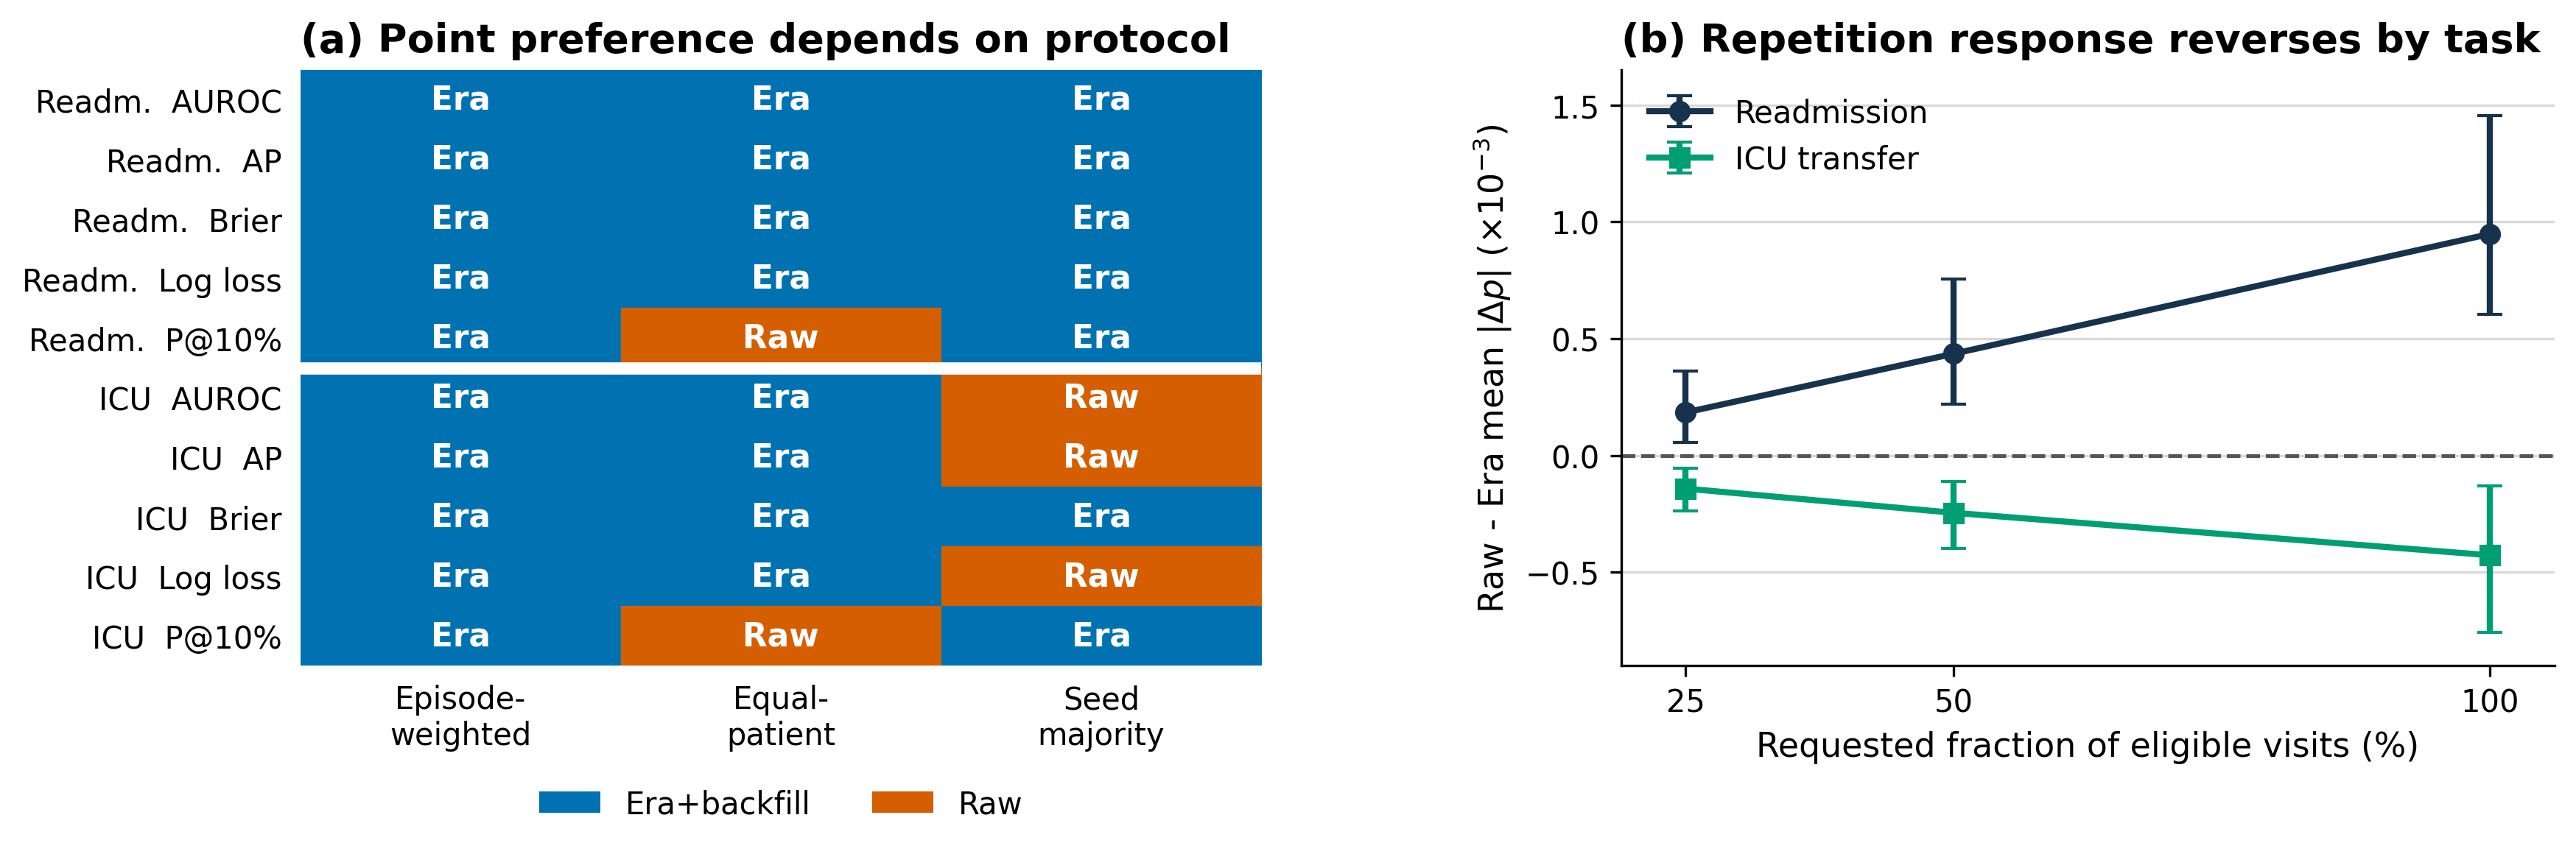
\includegraphics[width=0.90\linewidth]{figure_evaluation_profile.png}
  \caption{Protocol-dependent selection and repetition sensitivity. (a) Point
  preferences under episode weighting, equal-patient weighting, and seed
  majority; colors do not imply significance. (b) Raw minus Era+backfill mean
  absolute probability change under strict pre-prediction repetition, with
  paired patient-cluster 95\% intervals. Positive means Era+backfill changes less.}
  \label{fig:evaluation_profile}
\end{figure}

\paragraph{Episode-level membership changes.}
Table~\ref{tab:stress_churn} reports one entering and one exiting readmission
episode per pipeline and three of each for ICU. Strict eligible capacities are
129 and 103, versus 219 and 204 in the full cohorts. Raw loses one readmission
positive selection, while Era+backfill gains one; all ICU exchanges have negative
outcomes. These counts cannot support reliable subgroup inference or clinical
benefit claims.

\begin{table}[!htbp]
  \caption{Top-decile membership changes at 100\% requested repetition within
  strict eligible cohorts. Positive outcomes appear in parentheses; churn is
  exited episodes divided by $k$.}
  \label{tab:stress_churn}
  \centering
  \small
  \begin{tabular*}{\linewidth}{@{\extracolsep{\fill}}llrrrr@{}}
    \toprule
    Task & Pipeline & Top $k$ & Entered (pos.) & Exited (pos.) & Changed patients \\
    \midrule
    \multirow{2}{*}{Readm.}
      & Raw & 129 & 1 (0) & 1 (1) & 2 \\
      & Era+backfill & 129 & 1 (1) & 1 (0) & 2 \\
    \midrule
    \multirow{2}{*}{ICU}
      & Raw & 103 & 3 (0) & 3 (0) & 6 \\
      & Era+backfill & 103 & 3 (0) & 3 (0) & 4 \\
    \bottomrule
  \end{tabular*}
\end{table}

\paragraph{Tail changes and interpretation.}
At the 100\% intervention level, the largest 95th-percentile absolute
probability change across pipelines was 0.005739. The largest individual change,
0.097974, occurred for ICU Era+backfill and corresponds to approximately 9.8
percentage points. Table~\ref{tab:stress_shift_tail} characterizes the largest
5\% of shifts: eligible-visit medians are higher than in the remainder for
every pipeline, while candidate-mention differences vary by task and pipeline.

\begin{table}[!htbp]
  \caption{Largest-5\%-shift profiles at full repetition in strict stress
  cohorts. Mentions and eligible visits are medians: tail (remainder).
  Maximum $|\Delta p|$ is in percentage points (pp); selection is defined in Methods.}
  \label{tab:stress_shift_tail}
  \centering
  \footnotesize
  \begin{tabular*}{\linewidth}{@{\extracolsep{\fill}}llrrrr@{}}
    \toprule
    Task & Pipeline & $n_{\mathrm{tail}}$ & \shortstack{Mentions\\tail (remainder)}
      & \shortstack{Eligible visits\\tail (remainder)} & \shortstack{Max $|\Delta p|$\\pp} \\
    \midrule
    \multirow{2}{*}{Readmission}
      & Raw & 65 & 17 (6) & 71 (22) & 5.577 \\
      & Era+backfill & 65 & 5 (7) & 48 (22) & 3.306 \\
    \midrule
    \multirow{2}{*}{ICU transfer}
      & Raw & 52 & 8.5 (6) & 38 (24) & 4.065 \\
      & Era+backfill & 52 & 15 (6) & 59 (23) & 9.797 \\
    \bottomrule
  \end{tabular*}
\end{table}

At the 100\% requested level, eligible-visit count also determines the number
of inserted diagnoses, so visit-count enrichment combines history
characteristics with intervention dose.

Baseline Raw histories reach the event cap in 67.7\% and 60.0\% of the
readmission Raw/Era tails, and 61.5\% and 65.4\% of the ICU Raw/Era tails.
For ICU Era+backfill, median time since first candidate mention is 764 days
in the tail versus 383 in the remainder. These post-hoc, stress-conditional
associations characterize episodes with large shifts, not their causes or
clinical significance; tail membership does not imply top-decile entry or exit.
Small mean shifts and set churn therefore coexist with larger episode-level
sensitivity.

\FloatBarrier

\section{Discussion}

\paragraph{Cohort performance versus thresholded selection.}
Global metrics average over a cohort, whereas top-decile selection depends on
local ordering. Despite favorable point estimates, 15.5\% and 25.0\% of
selected episodes remain representation-specific after ensembling.
Table~\ref{tab:matched_size_stability} supplies descriptive retraining references,
not attribution. Equal-patient P@10 shows analysis-unit dependence; similar
cohort ECE neither explains discordance nor rules out local calibration differences.

\paragraph{Mechanisms of persistence-aware representation.}
Only 4.2\% of ICU and 5.8\% of readmission episodes gain an earlier retained
timestamp. Structure-null controls associate the clearest ICU gains with
explicit state, but the full-history contrast also changes era construction.
Context length and era horizon trade metrics rather than improving them uniformly.
Neither aggregate ablations nor the discordant profile in
Table~\ref{tab:discordant_characterization} explain the clinical causes of
selection changes. Persistence state, historical reach, context budget, and
era horizon remain distinct design choices.

\paragraph{Task-specific perturbation sensitivity.}
Controlled repetition is dampened by Era+backfill for readmission and amplified
for ICU, precluding one representation-wide robustness claim. The tail profile
in Table~\ref{tab:stress_shift_tail} links larger shifts to specific recorded
history characteristics, descriptively rather than causally. Stress membership
changes in Table~\ref{tab:stress_churn} use smaller eligible cohorts than the complete
held-out representation comparison, so their rates are not a matched
instability baseline. This frozen-pipeline test probes a specified
pre-prediction perturbation, not the prevalence or effect of real-world
copy-forward or the clinical significance of the affected histories.

\paragraph{Implications for thresholded model selection.}
For thresholded use, a compact profile should pair use-aligned metrics with
patient-cluster uncertainty, calibration, retraining variability, selected-set
agreement, and relevant behavioral tests. It should not collapse these into one
score: outcome, capacity, and primary metric define the decision, while the
other dimensions expose distinct failure modes. The same principle applies
whenever continuous scores become finite prioritization sets.

\section{Conclusion}

Similar cohort-level scores do not imply interchangeable high-risk
prioritization. Era+backfill leads every primary point estimate, component
controls locate an ICU signal in explicit state encoding, and the five-seed
ensembles still disagree at the same prioritization capacity. Paired uncertainty
and opposite repetition responses further show why aggregate ranking alone
cannot resolve the choice.

The scope is one EHR source, two outcomes, 85 positive ICU held-out episodes,
one architecture per task, and a 10\% prioritization capacity. Development used
held-out feedback across 81 variants per task; bootstrap intervals condition on fitted
ensembles, and tuning supports both stopping and calibration. Exact-time events,
opaque \texttt{CARE\_SITE} codes, and one repetition mechanism leave residual
proxy risk. Seeds vary initialization, not sampled training patients, and the
post-hoc profile covers only stress-eligible episodes; neither alternative-split
stability nor clinical causes of discordance are established.

A locked external cohort and preregistered protocol can test effect magnitudes,
selected sets, subgroup behavior, alternative thresholds and splits, and
clinical net benefit. The immediate contribution is a reproducible profile
that exposes when a small benchmark difference changes who receives priority.

\section*{Acknowledgments}
The study was supported by the Ministry of Economic Development of the Russian
Federation (agreement No. 139-10-2025-034 dd. 19.06.2025, IGK
000000C313925P4D0002).

\clearpage

\bibliographystyle{plainnat}
\bibliography{references}

\appendix

\section{Additional Experimental Details and Results}
\label{app:data_details}

\paragraph{Split integrity and temporal boundary.}
Nine saved checks cover expected split values, duplicate examples, patient
overlap, one-split-per-patient, one-split-per-row, agreement with official
subject assignments, cross-source consistency, row mapping, and label
coverage. All passed with zero issues, establishing the integrity of split and
row assignments. The final boundary is
$t_{\mathrm{event}}\leq t_{\mathrm{prediction}}$; these checks do not rule out
all temporal proxies or semantic leakage through opaque codes.
Table~\ref{tab:split_counts} gives the audited cohort counts.

\begin{table}[htbp]
  \caption{Episode, patient, and positive-outcome counts by official split.}
  \label{tab:split_counts}
  \centering
  \small
  \begin{tabular*}{\linewidth}{@{\extracolsep{\fill}}llrrr@{}}
    \toprule
    Task & Split & Episodes & Patients & Positives \\
    \midrule
    \multirow{3}{*}{Readmission}
      & Train & 2,608 & 1,337 & 370 \\
      & Tuning & 2,206 & 1,191 & 281 \\
      & Held-out & 2,189 & 1,190 & 260 \\
    \midrule
    \multirow{3}{*}{ICU transfer}
      & Train & 2,402 & 1,306 & 113 \\
      & Tuning & 2,052 & 1,157 & 92 \\
      & Held-out & 2,037 & 1,154 & 85 \\
    \bottomrule
  \end{tabular*}
\end{table}

\FloatBarrier

\paragraph{Persistence whitelist.}
The train split contains 2,295 subjects, of whom 2,094 have diagnosis events,
459,789 diagnosis events, and 6,736 unique diagnosis codes. The fixed rule in
Section 3 selects 239 codes.

\subsection{All ensemble metrics}

Table~\ref{tab:all_metrics} reports every final task--representation ensemble,
including the component and sensitivity variants summarized in the main text.

\begin{table}[htbp]
  \caption{Five-seed calibrated ensemble results for every final
  task--representation pair.}
  \label{tab:all_metrics}
  \centering
  \small
  \begin{tabular*}{\linewidth}{@{\extracolsep{\fill}}llrrrrr@{}}
    \toprule
    Task & Representation & AUROC & AP & Brier & Log loss & P@10\% \\
    \midrule
    \multirow{6}{*}{Readm.}
      & Raw 4096 & .7942 & .4097 & .08690 & .29956 & .4521 \\
      & Era+backfill 4096 & .7985 & .4206 & .08602 & .29693 & .4658 \\
      & Era no-backfill 4096 & .8007 & .4052 & .08710 & .29915 & .4703 \\
      & Era structure-null 4096 & .7928 & .4126 & .08688 & .29996 & .4566 \\
      & Raw 16384 & .8034 & .4202 & .08804 & .30562 & .4384 \\
      & Era+backfill 16384 & .7942 & .4161 & .08767 & .30342 & .4658 \\
    \midrule
    \multirow{8}{*}{ICU}
      & Raw 4096 & .7948 & .2194 & .03637 & .14926 & .1765 \\
      & Era+backfill 4096 & .8013 & .2241 & .03618 & .14745 & .1814 \\
      & Era no-backfill 4096 & .7732 & .2007 & .03682 & .15176 & .1667 \\
      & Era structure-null 4096 & .7704 & .1825 & .03731 & .15528 & .1569 \\
      & Raw 16384 & .7805 & .2017 & .03690 & .15305 & .1814 \\
      & Era+backfill 16384 & .7774 & .2352 & .03615 & .15053 & .1765 \\
      & Era+backfill gap30 & .7550 & .1601 & .03765 & .15565 & .1569 \\
      & Era+backfill gap180 & .7757 & .2362 & .03634 & .14995 & .1961 \\
    \bottomrule
  \end{tabular*}
\end{table}

\FloatBarrier

\subsection{Calibration curves}
\label{app:calibration_curves}

Figure~\ref{fig:calibration} visualizes the calibration summaries reported in
Table~\ref{tab:calibration_main} without adding a separate selection criterion.

\begin{figure}[htbp]
  \centering
  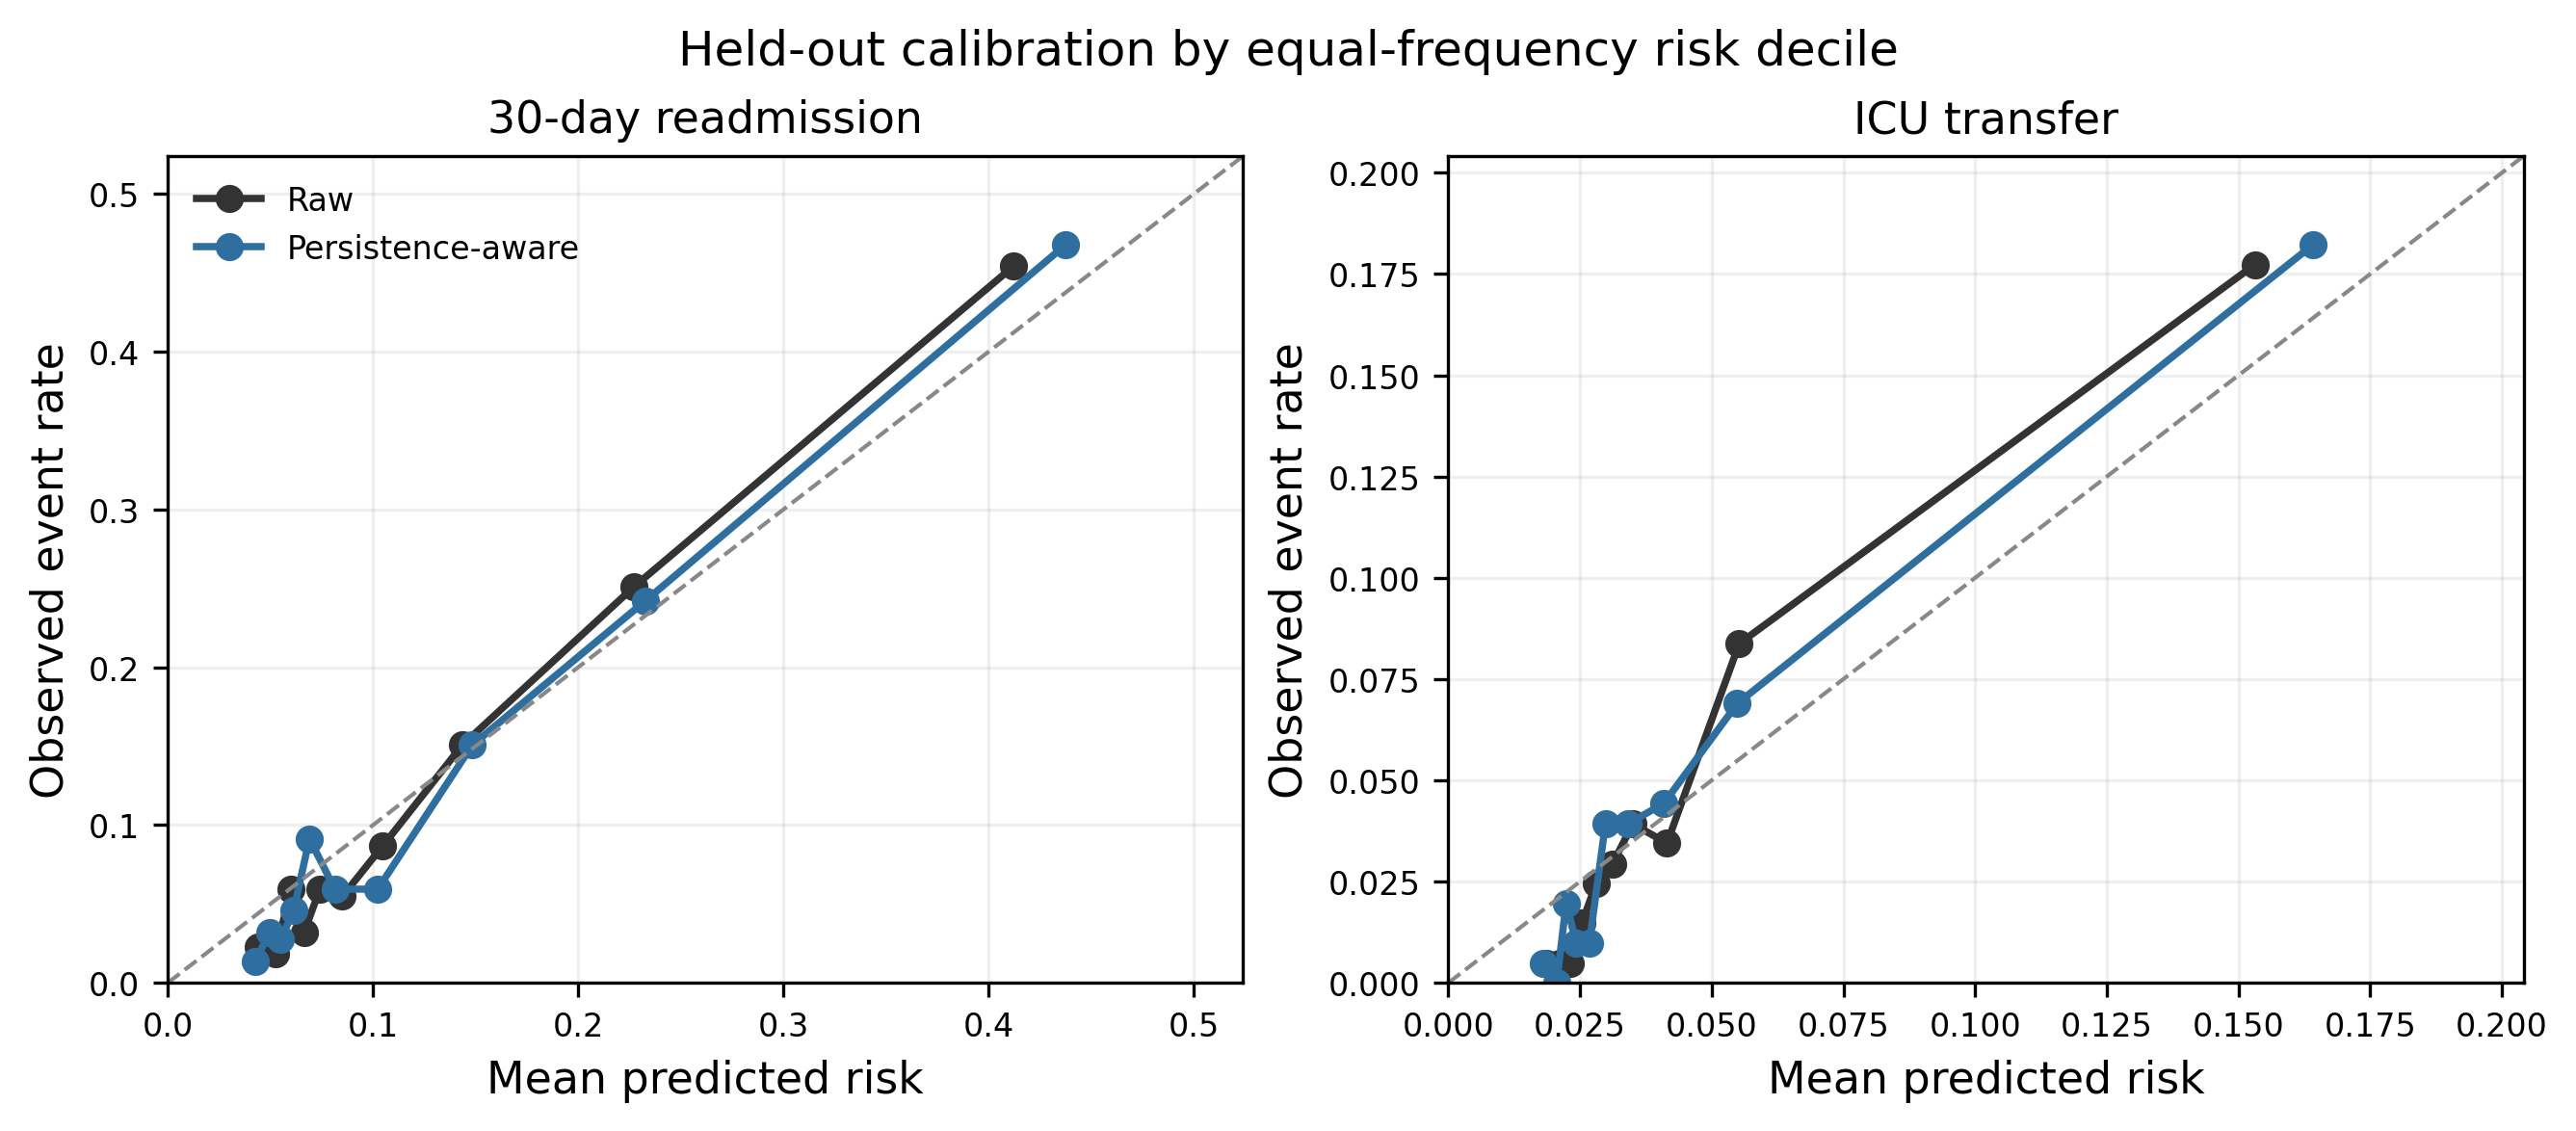
\includegraphics[width=0.88\linewidth]{figure_calibration_curves.png}
  \caption{Equal-frequency reliability curves for the four primary ensembles.
  Points plot observed outcome rate against mean predicted risk in ten held-out
  bins; the diagonal denotes perfect calibration. Bin-level intervals are not
  shown. Table~\ref{tab:calibration_main} reports ECE, intercept, slope, and
  patient-cluster intervals.}
  \label{fig:calibration}
\end{figure}

\FloatBarrier

\subsection{Seed-level summary}
\label{app:seed_summary}

Table~\ref{tab:seed_summary} separates ensemble-level comparisons from
variation across the five complete retraining runs.

\begin{table}[htbp]
  \caption{Mean $\pm$ SD across five independently trained seeds for the
  primary pipelines. Direction counts are Era+backfill/Raw/tie; lower is
  better for Brier and log loss.}
  \label{tab:seed_summary}
  \centering
  \small
  \begin{tabular*}{\linewidth}{@{\extracolsep{\fill}}llrrc@{}}
    \toprule
    Task & Metric & Raw & Era+backfill & Direction count \\
    \midrule
    \multirow{5}{*}{Readm.}
      & AUROC & $.7838\pm.0105$ & $.7866\pm.0102$ & 3/2/0 \\
      & AP & $.3834\pm.0273$ & $.3931\pm.0142$ & 3/2/0 \\
      & Brier & $.08922\pm.00201$ & $.08805\pm.00149$ & 4/1/0 \\
      & Log loss & $.30629\pm.00538$ & $.30282\pm.00526$ & 4/1/0 \\
      & P@10\% & $.4183\pm.0306$ & $.4384\pm.0168$ & 3/1/1 \\
    \midrule
    \multirow{5}{*}{ICU}
      & AUROC & $.7484\pm.0442$ & $.7636\pm.0164$ & 2/3/0 \\
      & AP & $.1833\pm.0396$ & $.1963\pm.0252$ & 2/3/0 \\
      & Brier & $.03762\pm.00081$ & $.03733\pm.00068$ & 3/2/0 \\
      & Log loss & $.15527\pm.00486$ & $.15285\pm.00335$ & 2/3/0 \\
      & P@10\% & $.1480\pm.0181$ & $.1706\pm.0220$ & 3/1/1 \\
    \bottomrule
  \end{tabular*}
\end{table}

\FloatBarrier

\subsection{Multiplicity sensitivity}

Twelve of 60 nominal \ci{}s exclude zero. Three Holm-adjusted and seven
Benjamini--Hochberg-adjusted bootstrap sign-tail quantities are below 0.05.
Both adjustments use the full family of 60 contrast--metric quantities.
Each quantity is twice the smaller bootstrap sign fraction with a Monte Carlo
$+1$ correction, based on 10,000 replicates. Its exact null calibration is not
guaranteed, the family was retrospective, and these adjusted values do not
provide confirmatory FWER or FDR control.

\subsection{Synthetic repetition results}

Table~\ref{tab:copy_forward} gives the requested repetition levels and paired
changes underlying Figure~\ref{fig:evaluation_profile}(b).

\begin{table}[htbp]
  \caption{Mean absolute probability change under strict pre-prediction
  synthetic repetition. Fractions are requested values; the number of changed
  visits is ceiling-rounded. The difference is Raw minus Era+backfill; positive
  values mean Era+backfill changes less.}
  \label{tab:copy_forward}
  \centering
  \small
  \begin{tabular*}{\linewidth}{@{\extracolsep{\fill}}lrrrr@{}}
    \toprule
    Task & Requested fraction & Raw & Era+backfill & Difference [\ci{}] \\
    \midrule
    Readm. & 25\% & .000408 & .000224 & .000184 [.000057, .000361] \\
    Readm. & 50\% & .000710 & .000274 & .000436 [.000219, .000755] \\
    Readm. & 100\% & .001275 & .000327 & .000948 [.000604, .001454] \\
    ICU & 25\% & .000099 & .000241 & $-.000142$ [$-.000236$, $-.000055$] \\
    ICU & 50\% & .000219 & .000465 & $-.000245$ [$-.000397$, $-.000110$] \\
    ICU & 100\% & .000471 & .000898 & $-.000427$ [$-.000756$, $-.000131$] \\
    \bottomrule
  \end{tabular*}
\end{table}

\FloatBarrier

The initial stress inference reproduces its own 0\% baseline exactly by
construction. Compared with the separately saved main-run baseline, maximum
absolute differences are 0.0050 in logit and 0.000344 in calibrated
probability, consistent with rebuilding inference on a different device. All
reported deltas use the within-stress 0\% baseline.

\paragraph{Artifact availability.}
Code, configurations, publication-safe aggregate tables, and execution
instructions are available at
\url{https://github.com/LvovDmitro/ehrshot-state-or-space}.
\texttt{python paper/reproduce\_public.py} verifies publication-safe aggregate
tables and regenerates the paper figures offline, without clinical credentials.
It does not retrain models or recompute row-level bootstrap or profile analyses;
those require credentialed EHRSHOT access and the restricted inputs. EHRSHOT
source records, subject identifiers, row-level predictions, and model checkpoints
are not redistributed. The exact upstream revision and checksum of the local
MEDS archive were not retained; reproduction is anchored to cohort counts,
split audits, and derived-artifact checksums.

The maintained release preserves original authorship and states its licensing
scope in \texttt{LICENSING.md}: no blanket software license has been assigned.
EHRSHOT and MEDS upstream code retain their own Apache-2.0 licenses, which do
not license this release or the clinical data. Access to EHRSHOT records remains
governed by the benchmark's Credentialed Health Data License.

% Required NeurIPS checklist inlined so the package contains one .tex file.
\section*{NeurIPS Paper Checklist}

\begin{enumerate}

\item {\bf Claims}
    \item[] Question: Do the main claims made in the abstract and introduction accurately reflect the paper's contributions and scope?
    \item[] Answer: \answerYes{}
    \item[] Justification: The claims match the two-task evaluation and distinguish observed rankings from paired uncertainty.
    \item[] Guidelines:
    \begin{itemize}
        \item The answer \answerNA{} means that the abstract and introduction do not include the claims made in the paper.
        \item The abstract and/or introduction should clearly state the claims made, including the contributions made in the paper and important assumptions and limitations. A \answerNo{} or \answerNA{} answer to this question will not be perceived well by the reviewers. 
        \item The claims made should match theoretical and experimental results, and reflect how much the results can be expected to generalize to other settings. 
        \item It is fine to include aspirational goals as motivation as long as it is clear that these goals are not attained by the paper. 
    \end{itemize}

\item {\bf Limitations}
    \item[] Question: Does the paper discuss the limitations of the work performed by the authors?
    \item[] Answer: \answerYes{}
    \item[] Justification: Section 6 states the data, selection, architecture, threshold, proxy, and validation scope.
    \item[] Guidelines:
    \begin{itemize}
        \item The answer \answerNA{} means that the paper has no limitation while the answer \answerNo{} means that the paper has limitations, but those are not discussed in the paper. 
        \item The authors are encouraged to create a separate ``Limitations'' section in their paper.
        \item The paper should point out any strong assumptions and how robust the results are to violations of these assumptions (e.g., independence assumptions, noiseless settings, model well-specification, asymptotic approximations only holding locally). The authors should reflect on how these assumptions might be violated in practice and what the implications would be.
        \item The authors should reflect on the scope of the claims made, e.g., if the approach was only tested on a few datasets or with a few runs. In general, empirical results often depend on implicit assumptions, which should be articulated.
        \item The authors should reflect on the factors that influence the performance of the approach. For example, a facial recognition algorithm may perform poorly when image resolution is low or images are taken in low lighting. Or a speech-to-text system might not be used reliably to provide closed captions for online lectures because it fails to handle technical jargon.
        \item The authors should discuss the computational efficiency of the proposed algorithms and how they scale with dataset size.
        \item If applicable, the authors should discuss possible limitations of their approach to address problems of privacy and fairness.
        \item While the authors might fear that complete honesty about limitations might be used by reviewers as grounds for rejection, a worse outcome might be that reviewers discover limitations that aren't acknowledged in the paper. The authors should use their best judgment and recognize that individual actions in favor of transparency play an important role in developing norms that preserve the integrity of the community. Reviewers will be specifically instructed to not penalize honesty concerning limitations.
    \end{itemize}

\item {\bf Theory assumptions and proofs}
    \item[] Question: For each theoretical result, does the paper provide the full set of assumptions and a complete (and correct) proof?
    \item[] Answer: \answerNA{}
    \item[] Justification: The paper contains no theoretical results.
    \item[] Guidelines:
    \begin{itemize}
        \item The answer \answerNA{} means that the paper does not include theoretical results. 
        \item All the theorems, formulas, and proofs in the paper should be numbered and cross-referenced.
        \item All assumptions should be clearly stated or referenced in the statement of any theorems.
        \item The proofs can either appear in the main paper or the supplemental material, but if they appear in the supplemental material, the authors are encouraged to provide a short proof sketch to provide intuition. 
        \item Inversely, any informal proof provided in the core of the paper should be complemented by formal proofs provided in appendix or supplemental material.
        \item Theorems and Lemmas that the proof relies upon should be properly referenced. 
    \end{itemize}

    \item {\bf Experimental result reproducibility}
    \item[] Question: Does the paper fully disclose all the information needed to reproduce the main experimental results of the paper to the extent that it affects the main claims and/or conclusions of the paper (regardless of whether the code and data are provided or not)?
    \item[] Answer: \answerYes{}
    \item[] Justification: Methods and appendices specify training and evaluation; \texttt{paper/reproduce\_public.py} verifies public aggregate tables and regenerates figures offline. Retraining and row-level recomputation require credentialed EHRSHOT access and restricted inputs; source-provenance limitations are stated. Code and instructions are available at \url{https://github.com/LvovDmitro/ehrshot-state-or-space}.
    \item[] Guidelines:
    \begin{itemize}
        \item The answer \answerNA{} means that the paper does not include experiments.
        \item If the paper includes experiments, a \answerNo{} answer to this question will not be perceived well by the reviewers: Making the paper reproducible is important, regardless of whether the code and data are provided or not.
        \item If the contribution is a dataset and\slash or model, the authors should describe the steps taken to make their results reproducible or verifiable. 
        \item Depending on the contribution, reproducibility can be accomplished in various ways. For example, if the contribution is a novel architecture, describing the architecture fully might suffice, or if the contribution is a specific model and empirical evaluation, it may be necessary to either make it possible for others to replicate the model with the same dataset, or provide access to the model. In general, releasing code and data is often one good way to accomplish this, but reproducibility can also be provided via detailed instructions for how to replicate the results, access to a hosted model (e.g., in the case of a large language model), releasing of a model checkpoint, or other means that are appropriate to the research performed.
        \item While NeurIPS does not require releasing code, the conference does require all submissions to provide some reasonable avenue for reproducibility, which may depend on the nature of the contribution. For example
        \begin{enumerate}
            \item If the contribution is primarily a new algorithm, the paper should make it clear how to reproduce that algorithm.
            \item If the contribution is primarily a new model architecture, the paper should describe the architecture clearly and fully.
            \item If the contribution is a new model (e.g., a large language model), then there should either be a way to access this model for reproducing the results or a way to reproduce the model (e.g., with an open-source dataset or instructions for how to construct the dataset).
            \item We recognize that reproducibility may be tricky in some cases, in which case authors are welcome to describe the particular way they provide for reproducibility. In the case of closed-source models, it may be that access to the model is limited in some way (e.g., to registered users), but it should be possible for other researchers to have some path to reproducing or verifying the results.
        \end{enumerate}
    \end{itemize}


\item {\bf Open access to data and code}
    \item[] Question: Does the paper provide open access to the data and code, with sufficient instructions to faithfully reproduce the main experimental results, as described in supplemental material?
    \item[] Answer: \answerNo{}
    \item[] Justification: Public code and aggregates at \url{https://github.com/LvovDmitro/ehrshot-state-or-space} support offline aggregate verification and figure regeneration. This combined item remains No because full retraining requires credentialed EHRSHOT records and restricted derivatives; public availability does not constitute a blanket software license.
    \item[] Guidelines:
    \begin{itemize}
        \item The answer \answerNA{} means that paper does not include experiments requiring code.
        \item Please see the NeurIPS code and data submission guidelines (\url{https://neurips.cc/public/guides/CodeSubmissionPolicy}) for more details.
        \item While we encourage the release of code and data, we understand that this might not be possible, so \answerNo{} is an acceptable answer. Papers cannot be rejected simply for not including code, unless this is central to the contribution (e.g., for a new open-source benchmark).
        \item The instructions should contain the exact command and environment needed to run to reproduce the results. See the NeurIPS code and data submission guidelines (\url{https://neurips.cc/public/guides/CodeSubmissionPolicy}) for more details.
        \item The authors should provide instructions on data access and preparation, including how to access the raw data, preprocessed data, intermediate data, and generated data, etc.
        \item The authors should provide scripts to reproduce all experimental results for the new proposed method and baselines. If only a subset of experiments are reproducible, they should state which ones are omitted from the script and why.
        \item At submission time, to preserve anonymity, the authors should release anonymized versions (if applicable).
        \item Providing as much information as possible in supplemental material (appended to the paper) is recommended, but including URLs to data and code is permitted.
    \end{itemize}


\item {\bf Experimental setting/details}
    \item[] Question: Does the paper specify all the training and test details (e.g., data splits, hyperparameters, how they were chosen, type of optimizer) necessary to understand the results?
    \item[] Answer: \answerYes{}
    \item[] Justification: Sections 3 and A report splits, preprocessing, architectures, optimization, seeds, calibration, metrics, and inference.
    \item[] Guidelines:
    \begin{itemize}
        \item The answer \answerNA{} means that the paper does not include experiments.
        \item The experimental setting should be presented in the core of the paper to a level of detail that is necessary to appreciate the results and make sense of them.
        \item The full details can be provided either with the code, in appendix, or as supplemental material.
    \end{itemize}

\item {\bf Experiment statistical significance}
    \item[] Question: Does the paper report error bars suitably and correctly defined or other appropriate information about the statistical significance of the experiments?
    \item[] Answer: \answerYes{}
    \item[] Justification: Five retraining seeds, paired patient-cluster intervals, and multiplicity sensitivity are reported.
    \item[] Guidelines:
    \begin{itemize}
        \item The answer \answerNA{} means that the paper does not include experiments.
        \item The authors should answer \answerYes{} if the results are accompanied by error bars, confidence intervals, or statistical significance tests, at least for the experiments that support the main claims of the paper.
        \item The factors of variability that the error bars are capturing should be clearly stated (for example, train/test split, initialization, random drawing of some parameter, or overall run with given experimental conditions).
        \item The method for calculating the error bars should be explained (closed form formula, call to a library function, bootstrap, etc.)
        \item The assumptions made should be given (e.g., Normally distributed errors).
        \item It should be clear whether the error bar is the standard deviation or the standard error of the mean.
        \item It is OK to report 1-sigma error bars, but one should state it. The authors should preferably report a 2-sigma error bar than state that they have a 96\% CI, if the hypothesis of Normality of errors is not verified.
        \item For asymmetric distributions, the authors should be careful not to show in tables or figures symmetric error bars that would yield results that are out of range (e.g., negative error rates).
        \item If error bars are reported in tables or plots, the authors should explain in the text how they were calculated and reference the corresponding figures or tables in the text.
    \end{itemize}

\item {\bf Experiments compute resources}
    \item[] Question: For each experiment, does the paper provide sufficient information on the computer resources (type of compute workers, memory, time of execution) needed to reproduce the experiments?
    \item[] Answer: \answerNo{}
    \item[] Justification: Model dimensions and optimization are reported, but historical hardware and runtime totals are unavailable.
    \item[] Guidelines:
    \begin{itemize}
        \item The answer \answerNA{} means that the paper does not include experiments.
        \item The paper should indicate the type of compute workers CPU or GPU, internal cluster, or cloud provider, including relevant memory and storage.
        \item The paper should provide the amount of compute required for each of the individual experimental runs as well as estimate the total compute. 
        \item The paper should disclose whether the full research project required more compute than the experiments reported in the paper (e.g., preliminary or failed experiments that didn't make it into the paper). 
    \end{itemize}
    
\item {\bf Code of ethics}
    \item[] Question: Does the research conducted in the paper conform, in every respect, with the NeurIPS Code of Ethics \url{https://neurips.cc/public/EthicsGuidelines}?
    \item[] Answer: \answerYes{}
    \item[] Justification: The study follows benchmark data-use terms, redistributes no restricted records, and limits clinical claims.
    \item[] Guidelines:
    \begin{itemize}
        \item The answer \answerNA{} means that the authors have not reviewed the NeurIPS Code of Ethics.
        \item If the authors answer \answerNo, they should explain the special circumstances that require a deviation from the Code of Ethics.
        \item The authors should make sure to preserve anonymity (e.g., if there is a special consideration due to laws or regulations in their jurisdiction).
    \end{itemize}


\item {\bf Broader impacts}
    \item[] Question: Does the paper discuss both potential positive societal impacts and negative societal impacts of the work performed?
    \item[] Answer: \answerYes{}
    \item[] Justification: Discussion identifies transparent prioritization as a benefit and redirected follow-up as a risk, with monitoring safeguards.
    \item[] Guidelines:
    \begin{itemize}
        \item The answer \answerNA{} means that there is no societal impact of the work performed.
        \item If the authors answer \answerNA{} or \answerNo, they should explain why their work has no societal impact or why the paper does not address societal impact.
        \item Examples of negative societal impacts include potential malicious or unintended uses (e.g., disinformation, generating fake profiles, surveillance), fairness considerations (e.g., deployment of technologies that could make decisions that unfairly impact specific groups), privacy considerations, and security considerations.
        \item The conference expects that many papers will be foundational research and not tied to particular applications, let alone deployments. However, if there is a direct path to any negative applications, the authors should point it out. For example, it is legitimate to point out that an improvement in the quality of generative models could be used to generate Deepfakes for disinformation. On the other hand, it is not needed to point out that a generic algorithm for optimizing neural networks could enable people to train models that generate Deepfakes faster.
        \item The authors should consider possible harms that could arise when the technology is being used as intended and functioning correctly, harms that could arise when the technology is being used as intended but gives incorrect results, and harms following from (intentional or unintentional) misuse of the technology.
        \item If there are negative societal impacts, the authors could also discuss possible mitigation strategies (e.g., gated release of models, providing defenses in addition to attacks, mechanisms for monitoring misuse, mechanisms to monitor how a system learns from feedback over time, improving the efficiency and accessibility of ML).
    \end{itemize}
    
\item {\bf Safeguards}
    \item[] Question: Does the paper describe safeguards that have been put in place for responsible release of data or models that have a high risk for misuse (e.g., pre-trained language models, image generators, or scraped datasets)?
    \item[] Answer: \answerNA{}
    \item[] Justification: No deployable clinical model or new sensitive dataset is released.
    \item[] Guidelines:
    \begin{itemize}
        \item The answer \answerNA{} means that the paper poses no such risks.
        \item Released models that have a high risk for misuse or dual-use should be released with necessary safeguards to allow for controlled use of the model, for example by requiring that users adhere to usage guidelines or restrictions to access the model or implementing safety filters. 
        \item Datasets that have been scraped from the Internet could pose safety risks. The authors should describe how they avoided releasing unsafe images.
        \item We recognize that providing effective safeguards is challenging, and many papers do not require this, but we encourage authors to take this into account and make a best faith effort.
    \end{itemize}

\item {\bf Licenses for existing assets}
    \item[] Question: Are the creators or original owners of assets (e.g., code, data, models), used in the paper, properly credited and are the license and terms of use explicitly mentioned and properly respected?
    \item[] Answer: \answerYes{}
    \item[] Justification: Original authorship is preserved, EHRSHOT data terms and upstream EHRSHOT/MEDS Apache-2.0 licenses are distinguished, and \texttt{LICENSING.md} states that no blanket software license has been assigned to the maintained release.
    \item[] Guidelines:
    \begin{itemize}
        \item The answer \answerNA{} means that the paper does not use existing assets.
        \item The authors should cite the original paper that produced the code package or dataset.
        \item The authors should state which version of the asset is used and, if possible, include a URL\@.
        \item The name of the license (e.g., CC-BY 4.0) should be included for each asset.
        \item For scraped data from a particular source (e.g., website), the copyright and terms of service of that source should be provided.
        \item If assets are released, the license, copyright information, and terms of use in the package should be provided. For popular datasets, \url{paperswithcode.com/datasets} has curated licenses for some datasets. Their licensing guide can help determine the license of a dataset.
        \item For existing datasets that are re-packaged, both the original license and the license of the derived asset (if it has changed) should be provided.
        \item If this information is not available online, the authors are encouraged to reach out to the asset's creators.
    \end{itemize}

\item {\bf New assets}
    \item[] Question: Are new assets introduced in the paper well documented and is the documentation provided alongside the assets?
    \item[] Answer: \answerYes{}
    \item[] Justification: The public repository at \url{https://github.com/LvovDmitro/ehrshot-state-or-space} documents source, analysis, configurations, environment, manifests, aggregate outputs, offline reproduction, and credentialed retraining requirements; \texttt{LICENSING.md} states the absence of a blanket license grant.
    \item[] Guidelines:
    \begin{itemize}
        \item The answer \answerNA{} means that the paper does not release new assets.
        \item Researchers should communicate the details of the dataset\slash code\slash model as part of their submissions via structured templates. This includes details about training, license, limitations, etc. 
        \item The paper should discuss whether and how consent was obtained from people whose asset is used.
        \item At submission time, remember to anonymize your assets (if applicable). You can either create an anonymized URL or include an anonymized zip file.
    \end{itemize}

\item {\bf Crowdsourcing and research with human subjects}
    \item[] Question: For crowdsourcing experiments and research with human subjects, does the paper include the full text of instructions given to participants and screenshots, if applicable, as well as details about compensation (if any)? 
    \item[] Answer: \answerNA{}
    \item[] Justification: The study involved no crowdsourcing or participant interaction.
    \item[] Guidelines:
    \begin{itemize}
        \item The answer \answerNA{} means that the paper does not involve crowdsourcing nor research with human subjects.
        \item Including this information in the supplemental material is fine, but if the main contribution of the paper involves human subjects, then as much detail as possible should be included in the main paper. 
        \item According to the NeurIPS Code of Ethics, workers involved in data collection, curation, or other labor should be paid at least the minimum wage in the country of the data collector. 
    \end{itemize}

\item {\bf Institutional review board (IRB) approvals or equivalent for research with human subjects}
    \item[] Question: Does the paper describe potential risks incurred by study participants, whether such risks were disclosed to the subjects, and whether Institutional Review Board (IRB) approvals (or an equivalent approval/review based on the requirements of your country or institution) were obtained?
    \item[] Answer: \answerNA{}
    \item[] Justification: The study used a deidentified benchmark and introduced no new participant interaction.
    \item[] Guidelines:
    \begin{itemize}
        \item The answer \answerNA{} means that the paper does not involve crowdsourcing nor research with human subjects.
        \item Depending on the country in which research is conducted, IRB approval (or equivalent) may be required for any human subjects research. If you obtained IRB approval, you should clearly state this in the paper. 
        \item We recognize that the procedures for this may vary significantly between institutions and locations, and we expect authors to adhere to the NeurIPS Code of Ethics and the guidelines for their institution. 
        \item For initial submissions, do not include any information that would break anonymity (if applicable), such as the institution conducting the review.
    \end{itemize}

\item {\bf Declaration of LLM usage}
    \item[] Question: Does the paper describe the usage of LLMs if it is an important, original, or non-standard component of the core methods in this research? Note that if the LLM is used only for writing, editing, or formatting purposes and does \emph{not} impact the core methodology, scientific rigor, or originality of the research, declaration is not required.
    %this research? 
    \item[] Answer: \answerNA{}
    \item[] Justification: LLMs were not an experimental or methodological component.
    \item[] Guidelines:
    \begin{itemize}
        \item The answer \answerNA{} means that the core method development in this research does not involve LLMs as any important, original, or non-standard components.
        \item Please refer to our LLM policy in the NeurIPS handbook for what should or should not be described.
    \end{itemize}

\end{enumerate}

\end{document}
